\documentclass{ximera}

%\usepackage{todonotes}

\newcommand{\todo}{}

\usepackage{esint} % for \oiint
\graphicspath{
{./}
{functionsOfSeveralVariables/}
{normalVectors/}
{lagrangeMultipliers/}
{vectorFields/}
{greensTheorem/}
{shapeOfThingsToCome/}
}


\usepackage{tkz-euclide}
\tikzset{>=stealth} %% cool arrow head
\tikzset{shorten <>/.style={ shorten >=#1, shorten <=#1 } } %% allows shorter vectors

\usetikzlibrary{backgrounds} %% for boxes around graphs
\usetikzlibrary{shapes,positioning}  %% Clouds and stars
\usetikzlibrary{matrix} %% for matrix
\usepgfplotslibrary{polar} %% for polar plots
\usetkzobj{all}
\usepackage[makeroom]{cancel} %% for strike outs
%\usepackage{mathtools} %% for pretty underbrace % Breaks Ximera
\usepackage{multicol}
\usepackage{pgffor} %% required for integral for loops


%% http://tex.stackexchange.com/questions/66490/drawing-a-tikz-arc-specifying-the-center
%% Draws beach ball
\tikzset{pics/carc/.style args={#1:#2:#3}{code={\draw[pic actions] (#1:#3) arc(#1:#2:#3);}}}



\usepackage{array}
\setlength{\extrarowheight}{+.1cm}   
\newdimen\digitwidth
\settowidth\digitwidth{9}
\def\divrule#1#2{
\noalign{\moveright#1\digitwidth
\vbox{\hrule width#2\digitwidth}}}





\newcommand{\RR}{\mathbb R}
\newcommand{\R}{\mathbb R}
\newcommand{\N}{\mathbb N}
\newcommand{\Z}{\mathbb Z}

%\newcommand{\sage}{\textsf{SageMath}}


%\renewcommand{\d}{\,d\!}
\renewcommand{\d}{\mathop{}\!d}
\newcommand{\dd}[2][]{\frac{\d #1}{\d #2}}
\newcommand{\pp}[2][]{\frac{\partial #1}{\partial #2}}
\renewcommand{\l}{\ell}
\newcommand{\ddx}{\frac{d}{\d x}}

\newcommand{\zeroOverZero}{\ensuremath{\boldsymbol{\tfrac{0}{0}}}}
\newcommand{\inftyOverInfty}{\ensuremath{\boldsymbol{\tfrac{\infty}{\infty}}}}
\newcommand{\zeroOverInfty}{\ensuremath{\boldsymbol{\tfrac{0}{\infty}}}}
\newcommand{\zeroTimesInfty}{\ensuremath{\small\boldsymbol{0\cdot \infty}}}
\newcommand{\inftyMinusInfty}{\ensuremath{\small\boldsymbol{\infty - \infty}}}
\newcommand{\oneToInfty}{\ensuremath{\boldsymbol{1^\infty}}}
\newcommand{\zeroToZero}{\ensuremath{\boldsymbol{0^0}}}
\newcommand{\inftyToZero}{\ensuremath{\boldsymbol{\infty^0}}}



\newcommand{\numOverZero}{\ensuremath{\boldsymbol{\tfrac{\#}{0}}}}
\newcommand{\dfn}{\textbf}
%\newcommand{\unit}{\,\mathrm}
\newcommand{\unit}{\mathop{}\!\mathrm}
\newcommand{\eval}[1]{\bigg[ #1 \bigg]}
\newcommand{\seq}[1]{\left( #1 \right)}
\renewcommand{\epsilon}{\varepsilon}
\renewcommand{\phi}{\varphi}


\renewcommand{\iff}{\Leftrightarrow}

\DeclareMathOperator{\arccot}{arccot}
\DeclareMathOperator{\arcsec}{arcsec}
\DeclareMathOperator{\arccsc}{arccsc}
\DeclareMathOperator{\si}{Si}
\DeclareMathOperator{\proj}{\vec{proj}}
\DeclareMathOperator{\scal}{scal}
\DeclareMathOperator{\sign}{sign}


%% \newcommand{\tightoverset}[2]{% for arrow vec
%%   \mathop{#2}\limits^{\vbox to -.5ex{\kern-0.75ex\hbox{$#1$}\vss}}}
\newcommand{\arrowvec}{\overrightarrow}
%\renewcommand{\vec}[1]{\arrowvec{\mathbf{#1}}}
\renewcommand{\vec}{\mathbf}
\newcommand{\veci}{{\boldsymbol{\hat{\imath}}}}
\newcommand{\vecj}{{\boldsymbol{\hat{\jmath}}}}
\newcommand{\veck}{{\boldsymbol{\hat{k}}}}
\newcommand{\vecl}{\boldsymbol{\l}}
\newcommand{\uvec}[1]{\mathbf{\hat{#1}}}
\newcommand{\utan}{\mathbf{\hat{t}}}
\newcommand{\unormal}{\mathbf{\hat{n}}}
\newcommand{\ubinormal}{\mathbf{\hat{b}}}

\newcommand{\dotp}{\bullet}
\newcommand{\cross}{\boldsymbol\times}
\newcommand{\grad}{\boldsymbol\nabla}
\newcommand{\divergence}{\grad\dotp}
\newcommand{\curl}{\grad\cross}
%\DeclareMathOperator{\divergence}{divergence}
%\DeclareMathOperator{\curl}[1]{\grad\cross #1}
\newcommand{\lto}{\mathop{\longrightarrow\,}\limits}

\renewcommand{\bar}{\overline}

\colorlet{textColor}{black} 
\colorlet{background}{white}
\colorlet{penColor}{blue!50!black} % Color of a curve in a plot
\colorlet{penColor2}{red!50!black}% Color of a curve in a plot
\colorlet{penColor3}{red!50!blue} % Color of a curve in a plot
\colorlet{penColor4}{green!50!black} % Color of a curve in a plot
\colorlet{penColor5}{orange!80!black} % Color of a curve in a plot
\colorlet{penColor6}{yellow!70!black} % Color of a curve in a plot
\colorlet{fill1}{penColor!20} % Color of fill in a plot
\colorlet{fill2}{penColor2!20} % Color of fill in a plot
\colorlet{fillp}{fill1} % Color of positive area
\colorlet{filln}{penColor2!20} % Color of negative area
\colorlet{fill3}{penColor3!20} % Fill
\colorlet{fill4}{penColor4!20} % Fill
\colorlet{fill5}{penColor5!20} % Fill
\colorlet{gridColor}{gray!50} % Color of grid in a plot

\newcommand{\surfaceColor}{violet}
\newcommand{\surfaceColorTwo}{redyellow}
\newcommand{\sliceColor}{greenyellow}




\pgfmathdeclarefunction{gauss}{2}{% gives gaussian
  \pgfmathparse{1/(#2*sqrt(2*pi))*exp(-((x-#1)^2)/(2*#2^2))}%
}


%%%%%%%%%%%%%
%% Vectors
%%%%%%%%%%%%%

%% Simple horiz vectors
\renewcommand{\vector}[1]{\left\langle #1\right\rangle}


%% %% Complex Horiz Vectors with angle brackets
%% \makeatletter
%% \renewcommand{\vector}[2][ , ]{\left\langle%
%%   \def\nextitem{\def\nextitem{#1}}%
%%   \@for \el:=#2\do{\nextitem\el}\right\rangle%
%% }
%% \makeatother

%% %% Vertical Vectors
%% \def\vector#1{\begin{bmatrix}\vecListA#1,,\end{bmatrix}}
%% \def\vecListA#1,{\if,#1,\else #1\cr \expandafter \vecListA \fi}

%%%%%%%%%%%%%
%% End of vectors
%%%%%%%%%%%%%

%\newcommand{\fullwidth}{}
%\newcommand{\normalwidth}{}



%% makes a snazzy t-chart for evaluating functions
%\newenvironment{tchart}{\rowcolors{2}{}{background!90!textColor}\array}{\endarray}

%%This is to help with formatting on future title pages.
\newenvironment{sectionOutcomes}{}{} 



%% Flowchart stuff
%\tikzstyle{startstop} = [rectangle, rounded corners, minimum width=3cm, minimum height=1cm,text centered, draw=black]
%\tikzstyle{question} = [rectangle, minimum width=3cm, minimum height=1cm, text centered, draw=black]
%\tikzstyle{decision} = [trapezium, trapezium left angle=70, trapezium right angle=110, minimum width=3cm, minimum height=1cm, text centered, draw=black]
%\tikzstyle{question} = [rectangle, rounded corners, minimum width=3cm, minimum height=1cm,text centered, draw=black]
%\tikzstyle{process} = [rectangle, minimum width=3cm, minimum height=1cm, text centered, draw=black]
%\tikzstyle{decision} = [trapezium, trapezium left angle=70, trapezium right angle=110, minimum width=3cm, minimum height=1cm, text centered, draw=black]
\title[Prerequisite Videos: ]{[Video] Piece-Wise Functions}
\author{Ben Sencindiver}

\outcome{Find function values of piece-wise functions, find domain/range of piece-wise functions, and graph piece-wise functions.}

\begin{document}
\begin{abstract}
   In this set of videos, we will work to understand how to find function values of piece-wise functions, how to find the domain and range of piece-wise functions, and how to graph piece-wise functions.
\end{abstract}
\maketitle

%% Question 1
\textbf{Question 1: Finding function values of piece-wise functions.}
\begin{question}
%% Labeling this expandable option
\begin{flushright}
{\color{blue}(\emph{Click the arrow to the right to see the first question.})}
\end{flushright}
\begin{center}
\begin{expandable}
\youtube{Egm75HO7gzs}
%% Multiple Choice Question 1
\begin{flushright}
{\color{blue}(\emph{Click the arrow to the right to see the question
posed at the end of the video.})}
\end{flushright}
\begin{expandable}
Find $f(1)$ when $f(x)$ is defined by
\[ f(x) = \begin{cases} 
      \frac{1}{2}x + \frac{3}{2} & x<1 \\
     x^2+3x - 6 & 1\leq x\leq 10 \\
      (x-1)(x+1) & x>10\\	
   \end{cases}. \]
\begin{multipleChoice}
\choice[correct]{$-2$}
\choice{$-1$}
\choice{$0$}
\choice{$1$}
\choice{$2$}
\choice{$f(1)$ is undefined}
\end{multipleChoice}
%% Example 1
\begin{flushright}
{\color{blue}(\emph{Click the arrow to the right to see an example.})}
\end{flushright}
\begin{expandable}
Example 1
\youtube{bkArouEU3g0}
\end{expandable}
\end{expandable}
\end{expandable}
\end{center}
\end{question}


%% Question 2
\textbf{Question 2: Finding the domain of a piece-wise function.}
\begin{question}
%% Labeling this expandable option
\begin{flushright}
{\color{blue}(\emph{Click the arrow to the right to see the second question.})}
\end{flushright}
\begin{center}
\begin{expandable}
\youtube{J6I0Jcaqiaw}
%% Multiple Choice Question 2
\begin{flushright}
{\color{blue}(\emph{Click the arrow to the right to see the  question
posed at the end of the video.})}
\end{flushright}
\begin{expandable}
What is the domain of $f(x)$ if $f(x)$ is defined by the expression below?\\

\[ f(x) = \begin{cases} 
      2x+13 & x<-3 \\
      \dfrac{x^2+1}{x+5} & -3< x\leq 1 \\
      \frac{-1}{x^2-4} & x> 1\\	
   \end{cases} \]
   
\begin{hint}

Are there any values of $x>1$ for which $\frac{-1}{x^2-4}$ is undefined?

\end{hint}

\begin{multipleChoice}
\choice{$(-\infty, -3)$}
\choice{$(-\infty, -3]$}
\choice{$(-3, 1)$}
\choice{$(-3, 1]$}
\choice{$[-3,-1]$}
\choice{$(1, \infty)$}
\choice{$[1, \infty)$}
\choice{$(-\infty, -3) \cup (-3, 1]$}
\choice{$(-3, 1] \cup (1, \infty)$}
\choice{$(-\infty, -3) \cup (-3, 1] \cup [1, \infty)$}
\choice{$(-\infty, -3) \cup (-3, -2) \cup (-2, 1] \cup (1, 2) \cup (2, \infty)$}
\choice[correct]{$(-\infty, -3) \cup (-3, 1] \cup (1, 2) \cup (2, \infty)$}
\end{multipleChoice}
%% Example 2
\begin{flushright}
{\color{blue}(\emph{Click the arrow to the right to see an example.})}
\end{flushright}
\begin{expandable}
Example 2
\youtube{BeeaOn6zSO8}
\end{expandable}
\end{expandable}
\end{expandable}
\end{center}
\end{question}


%% Question 3
\textbf{Question 3: Find the range of a piece-wise function.}
\begin{question}
%% Labeling this expandable option
\begin{flushright}
{\color{blue}(\emph{Click the arrow to the right to see the third question.}) }
\end{flushright}
\begin{center}
\begin{expandable}
\youtube{QLNZW-_cLeM}
%% Multiple Choice Question 3
\begin{flushright}
{\color{blue}(\emph{Click the arrow to the right to see the question
posed at the end of the video.})}
\end{flushright}
\begin{expandable}

What is the range of $f(x)$ when $f(x)$ is defined by the expression below?\\

\[ f(x) = \begin{cases} 
      2x+3 & x<-3 \\
      x^2 & -3\leq x< 2 \\
      -1 & x> 3\\	
   \end{cases} \]
   
\begin{multipleChoice}
\choice{$(\infty, -3) \cup [0,9]$}
\choice{$(\infty, -3] \cup [4,9]$}
\choice{$(\infty, -1] \cup [0,9]$}
\choice[correct]{$(\infty, -3) \cup \{-1\} \cup [0,9]$}
\choice{$(\infty, -3) \cup \{-1\} \cup [0,9)$}
\end{multipleChoice}
%% Example 3
\begin{flushright}
{\color{blue}(\emph{Click the arrow to the right to see an example.})}
\end{flushright}
\begin{expandable}
Example 3
\youtube{tjn-DyPJhQA}
\end{expandable}
\end{expandable}
\end{expandable}
\end{center}
\end{question}


%% Question 4
\textbf{Question 4: Graphing piece-wise functions.}
\begin{question}
%% Labeling this expandable option
\begin{flushright}
{\color{blue}(\emph{Click the arrow to the right to see the fourth question.})}
\end{flushright}
\begin{center}
\begin{expandable}
\youtube{_3zhjq1uyEc}
%% Multiple Choice Question 4
\begin{flushright}
{\color{blue}(\emph{Click the arrow to the right to see the question
posed at the end of the video.})}
\end{flushright}
\begin{expandable}
Which of the graphs is the graph of $f(x)$ where $f(x)$ is defined below?
\[ f(x) = \begin{cases} 
      x^2-1 & x \leq 0 \\
     \frac{1}{3} x + 2 & 0< x \leq 3 \\
    4 & x>3.5
   \end{cases} \]
   
\begin{multicols}{2}
\begin{center}
A.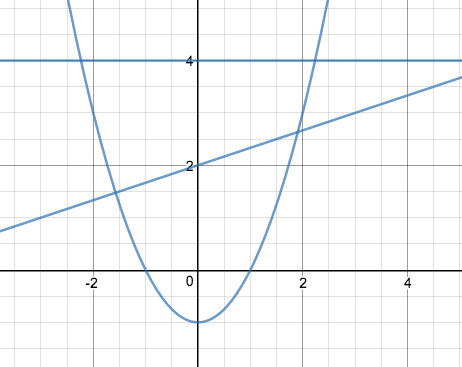
\includegraphics[scale=0.2]{PWGraph1}
\end{center}

\begin{center}
B. 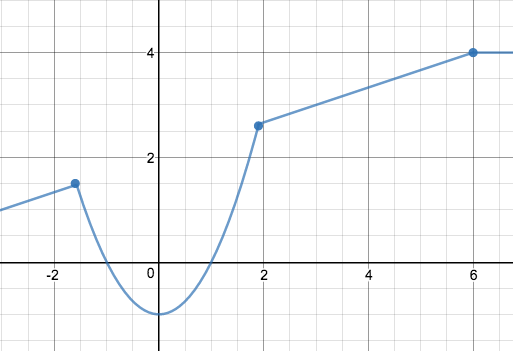
\includegraphics[scale=0.18]{PWGraph6}
\end{center}
\end{multicols}

\begin{multicols}{2}
\begin{center}
C. 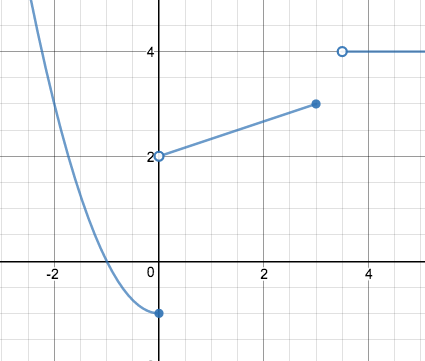
\includegraphics[scale=0.18]{PWGraph2}
\end{center}

\begin{center}
D. 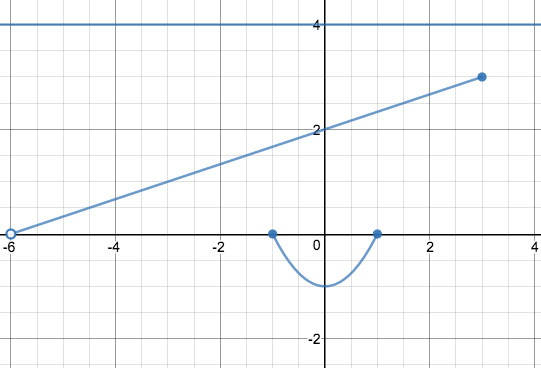
\includegraphics[scale=0.2]{PWGraph5}
\end{center}

\end{multicols}

\begin{center}
E.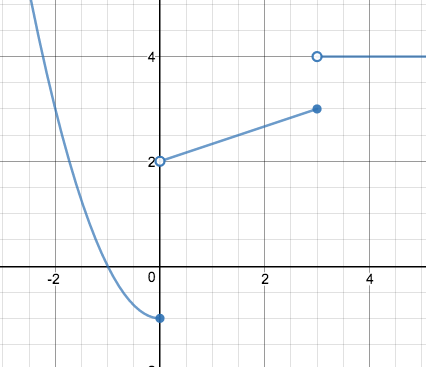
\includegraphics[scale=0.18]{PWGraph4}
\end{center}

\begin{multipleChoice}
\choice{A}
\choice{B}
\choice[correct]{C}
\choice{D}
\choice{E}
\choice{None of the above.}
\end{multipleChoice}
%% Example 4
\begin{flushright}
{\color{blue}(\emph{Click the arrow to the right to see an example.})}
\end{flushright}
\begin{expandable}
Example 4
\youtube{dq24Kyw7XTU}
\end{expandable}
\end{expandable}
\end{expandable}
\end{center}
\end{question}

\end{document}

